\documentclass{standalone}

\usepackage{tikz}
\usetikzlibrary{arrows}
\usetikzlibrary{decorations.markings}
\usetikzlibrary{calc}

\begin{document}

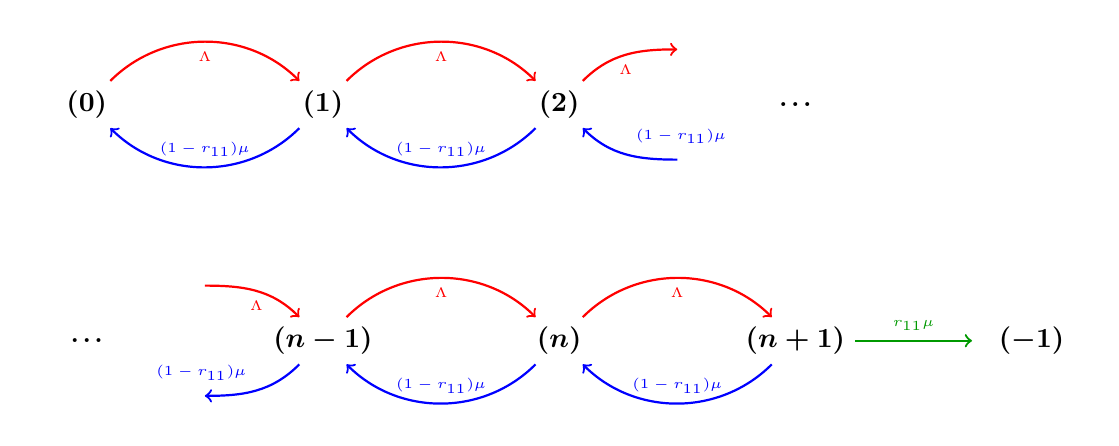
\begin{tikzpicture}
    \tikzstyle{state}=[minimum width=1.5cm, font=\boldmath];
    % First row
    \node (0) at (0,0) [state] {$(0)$};
    \node (1) at ($(0)+(3,0)$) [state] {$(1)$};
    \node (2) at ($(1)+(3,0)$) [state] {$(2)$};
    \node (dots1) at ($(2)+(3,0)$) [state] {\LARGE...};

    % Second row
    \node (dots2) at ($(0)+(0,-3)$) [state] {\LARGE...};
    \node (n-1) at ($(1)+(0,-3)$) [state] {$(n-1)$};
    \node (n) at ($(n-1)+(3,0)$) [state] {$(n)$};
    \node (n+1) at ($(n)+(3,0)$) [state] {$(n+1)$};
    \node (-1) at ($(n+1)+(3,0)$) [state] {$(-1)$};

    % Transitions
    % Arrivals

    \draw[draw=red] (0) edge[out=45,in=135,->,thick] node [below, text=red] {\tiny$\Lambda$}  (1);
    \draw[draw=red] (1) edge[out=45,in=135,->,thick] node [below, text=red] {\tiny$\Lambda$}  (2);
    \draw[draw=red] (2) edge[out=45,in=180,->,thick] node [below, text=red] {\tiny$\Lambda$}  ($(2)+(1.5,0.7)$);
    \draw[draw=red] ($(n-1)+(-1.5,0.7)$) edge[out=0,in=135,->,thick] node [below, text=red] {\tiny$\Lambda$}  (n-1);
    \draw[draw=red] (n-1) edge[out=45,in=135,->,thick] node [below, text=red] {\tiny$\Lambda$}  (n);
    \draw[draw=red] (n) edge[out=45,in=135,->,thick] node [below, text=red] {\tiny$\Lambda$}  (n+1);

    % Services

    \draw[draw=blue] (0) edge[out=-45,in=-135,<-,thick] node [above, text=blue] {\tiny$(1-r_{11})\mu$} (1);
    \draw[draw=blue] (1) edge[out=-45,in=-135,<-,thick] node [above, text=blue] {\tiny$(1-r_{11})\mu$} (2);
    \draw[draw=blue] (2) edge[out=-45,in=180,<-,thick] node [above right, text=blue] {\tiny$(1-r_{11})\mu$} ($(2)+(1.5,-0.7)$);
    \draw[draw=blue] ($(n-1)+(-1.5,-0.7)$) edge[out=0,in=-135,<-,thick] node [above left, text=blue] {\tiny$(1-r_{11})\mu$} (n-1);
    \draw[draw=blue] (n-1) edge[out=-45,in=-135,<-,thick] node [above, text=blue] {\tiny$(1-r_{11})\mu$} (n);
    \draw[draw=blue] (n) edge[out=-45,in=-135,<-,thick] node [above, text=blue] {\tiny$(1-r_{11})\mu$} (n+1);

    % To deadlock

    \draw[draw=green!60!black] (n+1) edge[->,thick] node [above, text=green!60!black] {\tiny$r_{11}\mu$} (-1);

\end{tikzpicture}

\end{document}
